%%%%
% Consiglio la visione dei seguenti tutorial:
% - https://www.youtube.com/watch?v=ihxSUsJB_14
% - https://www.youtube.com/watch?v=XTFWaV55uDo
%%%%
\documentclass[12pt,a4paper,openright,twoside]{book}
\usepackage[utf8]{inputenc}

%\newcommand{\thesislang}{italian} % decommentare in caso di tesi in italiano
\newcommand{\thesislang}{english} % commentare in caso di tesi in italiano
\usepackage{thesis-style}
% version
\newcommand{\versionmajor}{0}
\newcommand{\versionminor}{1}
\newcommand{\versionpatch}{2}
\newcommand{\version}{\versionmajor.\versionminor.\versionpatch}
\typeout{Document version: \version}

\begin{document}
	
\frontmatter

% ! TeX root = thesis-main.tex
\title{Title}
\author{Candidate Name Here}
\date{\today}

\newgeometry{margin=0.8in}
\begin{titlepage}
	\begin{center}
		% \vspace*{0.2cm}
		
		\large
		\textbf{ALMA MATER STUDIORUM -- UNIVERSITÀ DI BOLOGNA \\ CAMPUS DI CESENA}
		\\
		\noindent\hrulefill
		\vspace{0.4cm}
		
		\Large
		Scuola di Ingegneria e Architettura \\
		Corso di Laurea (Magistrale) in Ingegneria e Scienze Informatiche
		
		\Huge
		\vspace{4cm}
		\textbf{
			Fair-by-design matching algorithm
		}
		
		\large
		\vspace{1cm}
		Tesi di laurea in 
		\\
		\textsc{(Intelligent System Engineering)}
		
		\vspace{5.5cm}
		\begin{minipage}[t]{0.64\textwidth}
			\begin{flushleft}
				\textit{Relatore} 
				\\ 
				(\textbf{Prof.} $\mid$ \textbf{Dott.}) \textbf{Nome Cognome}
				\\
				\vspace{0.4cm}
				\textit{Correlatore} 
				\\
				(\textbf{Ing.})? \textbf{Dott.} \textbf{Nome Cognome}
			\end{flushleft}
		\end{minipage}
		\begin{minipage}[t]{0.34\textwidth}
			\begin{flushright}
				\textit{Candidato} 
				\\ 
				\textbf{Antonio Iannotta}
			\end{flushright}
		\end{minipage}\\
		
		\vfill
		\noindent\hrulefill
		\vspace{0.3cm}
		\Large
		
		%(N-Esima) Sessione di Laurea
		II Sessione di Laurea
		\\
		Anno Accademico 2022-2023
	\end{center}
\end{titlepage}
\restoregeometry


\begin{abstract}	
Artificial Intelligence (AI) has revolutionized many sectors, including matching, by providing automated solutions for resource, opportunity, or information associations. However, the widespread use of matching algorithms in AI can also lead to potential discrimination, amplifying existing inequalities in society. This thesis focuses on the development of fair-by-design algorithms for matching in the field of artificial intelligence to ensure ethical, transparent, and non-discriminatory association decisions.

Throughout the research, various fundamental aspects of matching in the context of AI and the associated ethical implications are examined. The main challenges related to discrimination, fairness, and transparency in the matching process are identified. Subsequently, the current approaches and methodologies available for developing fair-by-design algorithms are presented and analyzed.

The thesis proposes a novel approach to matching that integrates fairness and discrimination criteria within the algorithmic process. Different fairness and discrimination metrics are explored to assess the impact of matching algorithms on the distribution of opportunities and equitable treatment of different user categories.

The implementation of fair-by-design algorithms for matching is evaluated through a series of case studies, where the performance of the proposed algorithms is analyzed and compared to conventional solutions. The results demonstrate that fair-by-design algorithms can significantly reduce disparities and discrimination compared to traditional matching methods.

Finally, guidelines are proposed for developers and stakeholders interested in matching in the field of AI, aiming to promote the adoption of fair-by-design algorithms and encourage ethical and responsible use of artificial intelligence.
\end{abstract}

\begin{dedication} % this is optional
Optional. Max a few lines.
\end{dedication}

\begin{acknowledgements} % this is optional
Optional. Max 1 page.
\end{acknowledgements}

%----------------------------------------------------------------------------------------
\tableofcontents   
\listoffigures     % (optional) comment if empty
\lstlistoflistings % (optional) comment if empty
%----------------------------------------------------------------------------------------

\mainmatter

%----------------------------------------------------------------------------------------
\chapter{\introductionname}
\label{chap:introduction}
%----------------------------------------------------------------------------------------

%Write introduction here.

\section{Background}
In recent years, artificial intelligence (AI) systems have become pervasive in our society. From online product recommendations to healthcare, from industrial automation to autonomous vehicles, AI algorithms have become an integral part of many applications and services we use on a daily basis. These systems are capable of processing large amounts of data, recognizing complex patterns, and making autonomous decisions or supporting human decision-making.
However, while AI offers countless opportunities and advantages, it also raises concerns about the impact it can have on society. In particular, the widespread adoption of AI algorithms has led to increased discussions about fairness and discrimination within these systems.

\section{Fairness in AI}
Fairness is a central concept when it comes to AI systems. It refers to the need to ensure that such systems are unbiased and non-discriminatory towards the individuals or groups they affect. This is particularly relevant when considering the broad penetration and impact of AI systems in our society.
Fairness in AI systems can be approached from various perspectives. For example, when discussing fairness in hiring algorithms, it is crucial to ensure that hiring decisions are not influenced by gender bias or other personal characteristics. In resource allocation applications, such as educational scholarships, fairness implies that allocation decisions are based on merit and do not favor any specific group.
The relevance of fairness in AI systems also extends to issues of transparency and accountability. It is important that AI algorithms are understandable and explainable so that individuals can understand how decisions affecting them are made and can challenge any discrimination or bias.
Furthermore, fairness in AI systems has ethical and legal implications. Regulations such as the General Data Protection Regulation (GDPR) in the European Union require that automated decisions concerning individuals are subject to explanation, and anti-discrimination laws prohibit unfair discrimination based on protected characteristics such as race, gender, or religion.

\subsection{Types of Fairness}

In the context of artificial intelligence (AI) systems, there are several types of fairness that can be considered when developing algorithms that aim to ensure equitable distribution of resources or opportunities. The following are the main types of fairness:

\subsection{Statistical Fairness}
Statistical fairness is a critical concept in ensuring fairness in artificial intelligence (AI) systems. It aims to address the issue of disparate impacts on different demographic groups or protected categories when using AI algorithms. The goal of statistical fairness is to ensure that the outcomes produced by an AI algorithm are distributed fairly across these groups.

To achieve statistical fairness, it is important to examine the distribution of outcomes among different groups and identify any disparities. This can be done by analyzing the data used to train the AI algorithm and evaluating the resulting predictions or decisions.

There are several metrics and approaches that can be used to measure statistical fairness. These include:

\subsection{Disparate Impact}

Disparate Impact is a widely used concept and metric in the context of fairness assessment and evaluation of artificial intelligence (AI) systems. It refers to a situation where an AI algorithm has a significantly different impact on different demographic groups or protected categories, resulting in unequal outcomes. Disparate impact is a critical concern in ensuring fairness in AI systems and addressing potential biases.

\subsection{Measuring Disparate Impact}

Disparate Impact can be quantified using various statistical measures. One commonly used metric is the \textit{disparate impact ratio}, which is calculated by comparing the proportion of favorable outcomes for different groups. The disparate impact ratio is typically calculated by dividing the proportion of favorable outcomes for one group by the proportion for another group. If the ratio is close to 1, it suggests that the outcomes are fairly distributed, while a ratio significantly different from 1 indicates potential disparities.

Another commonly used measure is the \textit{between-group disparity}, which compares the absolute difference in favorable outcomes between groups. This measure provides a more nuanced understanding of the disparities and can be useful in identifying specific groups that are disproportionately affected.

\subsection{Legal Framework}

Disparate Impact has legal implications in many jurisdictions, particularly in the context of anti-discrimination laws. In the United States, for example, Title VII of the Civil Rights Act prohibits employment practices that have a disparate impact on protected groups, unless the practices are job-related and consistent with business necessity. This legal framework recognizes the importance of addressing systemic biases and promoting equal opportunities.

\subsection{Equalized Odds}

Equalized odds is another approach to statistical fairness that focuses on ensuring equal error rates across different groups. It requires that the true positive rates and false positive rates are similar for all groups. By achieving equalized odds, the algorithm aims to avoid privileging one group over another in terms of either false positives or false negatives. This approach is commonly used in applications such as criminal justice, where it is crucial to avoid both false convictions and false acquittals.

\subsection{Conditional Demographic Disparity}

Conditional demographic disparity is a metric that takes into account the demographic characteristics of individuals in relation to the predicted outcomes. It measures the difference in outcomes between different groups, considering individual attributes such as race, gender, or age. This metric allows for a more nuanced evaluation of fairness, as it considers how outcomes vary based on specific characteristics.

\subsection{Fairness-aware Algorithms}

To achieve statistical fairness, researchers and practitioners have developed fairness-aware algorithms. These algorithms aim to mitigate bias and disparities in the outcomes of AI systems by incorporating fairness constraints or objectives into the algorithm's optimization process. Fairness-aware algorithms seek to strike a balance between fairness and accuracy, ensuring that the predictions or decisions are both unbiased and effective.

However, it is important to note that achieving statistical fairness can be challenging. There may be trade-offs between fairness and other desirable properties, such as accuracy or efficiency. Balancing these trade-offs requires careful consideration and decision-making.

\subsection{Individual Fairness}
Individual fairness focuses on treating individuals with similar characteristics equally. The fundamental idea is that two individuals with similar features should receive similar treatment from the AI algorithm. For instance, in a personnel selection algorithm, individual fairness demands that two candidates with similar skills and qualifications have similar probabilities of being selected.

\subsection{Group Fairness}
Group fairness refers to equity in the treatment of specific groups of individuals defined by protected characteristics such as race, gender, or religion. The goal is to ensure that members of these groups have equal opportunities or benefits compared to other groups. For example, in an educational resource allocation algorithm, group fairness requires that each group has a fair share of allocated resources.

\subsection{Other Notions of Fairness}
In addition to the aforementioned types of fairness, there are other notions of fairness that can be considered in specific contexts. These include:

\begin{itemize}
    \item \textbf{Temporal Fairness}: Temporal fairness refers to the stability of decisions made over time. For instance, if an AI algorithm makes different decisions for the same individuals at different times, it may be deemed unfair.

    \item \textbf{Causal Fairness}: Causal fairness focuses on the causal effects of decisions made by AI algorithms. It aims to ensure that decisions do not perpetuate or amplify existing inequalities.

    \item \textbf{Process Fairness}: Process fairness pertains to the transparency and accessibility of the decision-making process of AI algorithms. It involves ensuring that the decision-making process is fair and comprehensible to individuals impacted by it.

    \item \textbf{Interpretability Fairness}: Interpretability fairness concerns the transparency and interpretability of AI algorithms. It involves making the decision-making process of AI systems interpretable to stakeholders and affected individuals, thereby promoting fairness.

    \item \textbf{Procedural Fairness}: Procedural fairness focuses on the fairness of the procedures followed in designing, training, and deploying AI algorithms. It involves ensuring that the entire process is fair, inclusive, and representative.

\end{itemize}


\section{Matching Algorithms}
Matching algorithms play a crucial role in various applications of AI. They involve the assignment of resources, individuals, or opportunities to optimize specific objectives. Common types of matching algorithms include the stable marriage algorithm, bipartite graph matching, and recommendation systems. These algorithms often rely on historical data or user preferences to make matches, which can introduce biases and perpetuate existing societal inequalities.

\subsection{Challenges in Fairness for Matching Algorithms}
Applying fairness to matching algorithms introduces unique challenges. One key challenge is the trade-off between fairness and optimizing matching outcomes. Striking a balance between these objectives requires careful algorithm design and considerations of fairness metrics. Additionally, addressing potential biases in the data used by the algorithms is crucial for achieving fair outcomes.

\section{Impact of Fairness in AI Systems on Society}
The fairness of AI systems, including matching algorithms, has a profound impact on society. Biased or discriminatory outcomes in matching can perpetuate and reinforce existing inequalities. For example, biased job matching algorithms may favor certain demographic groups, resulting in limited opportunities for others. Unfairness in important domains such as education, employment, or housing can have long-lasting effects on individuals and communities. It is essential to develop fair-by-design algorithms to mitigate these negative consequences and promote equal opportunities.

\subsection{Ethical Considerations}
Developing fair-by-design algorithms requires careful consideration of ethical implications. Fairness should not be pursued at the expense of other ethical principles such as privacy, transparency, or accountability. Striking the right balance between fairness and other considerations is vital to ensure the responsible implementation of matching algorithms.

\section{Thesis Objectives}
This thesis aims to explore the implementation of fair-by-design algorithms for matching and their impact on ensuring fairness in AI systems. The specific objectives are:

\begin{itemize}
    \item Investigate different fairness metrics and criteria applicable to matching algorithms.
    \item Develop novel fair-by-design algorithms for matching that balance fairness and optimization objectives.
    \item Assess the performance and effectiveness of the proposed fair-by-design algorithms through empirical evaluations and case studies.
    \item Analyze the societal impact of fair matching algorithms and the potential benefits of integrating fairness into AI systems.
\end{itemize}


%
\paragraph{Thesis Structure.} % Optional paragraph title
%

(This is optional an optional paragraph.)
%
Accordingly, the reminder of this thesis is structures as follows.
%
\Cref{chap:background} discusses (briefly describe the content of \cref{chap:background}).
%
Describe other chapters here in a similar way.
%
Finally, \Cref{chap:conclusions} concludes this thesis by summarising its main contribution.

%----------------------------------------------------------------------------------------
\chapter{State of the Art} % or Background
\label{chap:background}
%----------------------------------------------------------------------------------------

%Write background here.

%This section is likely to contain a lot of citations.
%
%For instance in \cite{AnzengruberSocInfo2013} the authors propose a novel means for tackling with the problem of preventing bad things from happening.

%----------------------------------------------------------------------------------------
\chapter{Design} % possible chapter for Projects
\label{chap:design}
%----------------------------------------------------------------------------------------

Write design here.

\begin{figure}
	\centering
	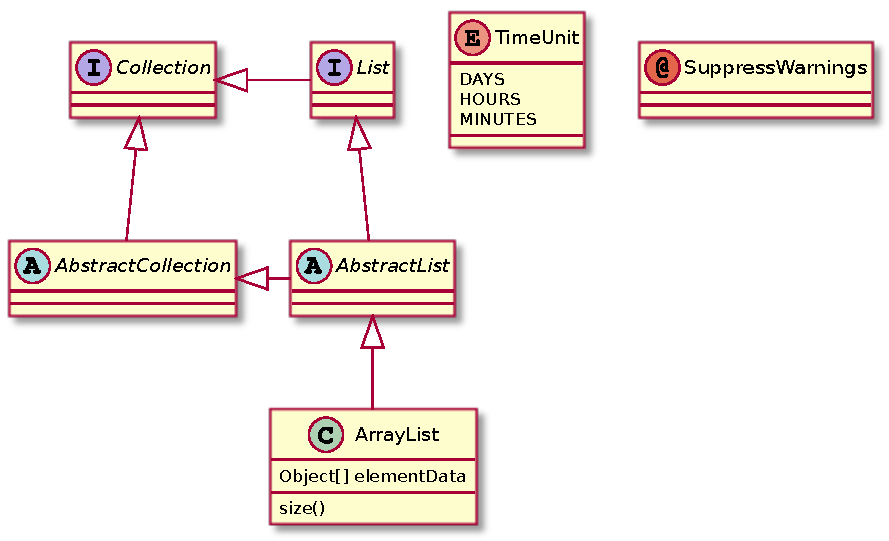
\includegraphics[width=0.5\linewidth]{figures/classes.pdf}
	\caption{A class diagram created with PlantUML}
	\label{fig:classes}
\end{figure}

You may want to reference images in your thesis.
%
In this case, you are encouraged to make them \emph{floating}, and reference them by means of labels.
%
For instance, in \Cref{fig:classes}, we describe a class diagram produced by means of \href{http://plantuml.com}{PlantUML}.

%----------------------------------------------------------------------------------------
\chapter{Implementation} % possible chapter for Projects
\label{chap:implementation}
%----------------------------------------------------------------------------------------

Write implementation here.

\lstinputlisting[
	float,
	language=Java,
	caption={My very first program in Java},
	label={lst:helloworld},
]{listings/HelloWorld.java}

You may need to reference listings in your thesis.
%
In this case, you are encouraged to make them \emph{floating}, and reference them by means of labels.
%
For instance, in \Cref{lst:helloworld}, we describe an hello world program in Java.

%----------------------------------------------------------------------------------------
\chapter{Validation} % possible chapter for Projects
\label{chap:validation}
%----------------------------------------------------------------------------------------

Write implementation here

%----------------------------------------------------------------------------------------
\chapter{\conclusionsname}
\label{chap:conclusions}
%----------------------------------------------------------------------------------------

Write conclusions here.


%----------------------------------------------------------------------------------------
% BIBLIOGRAPHY
%----------------------------------------------------------------------------------------

\nocite{*} % uncomment this to show all the reference in the .bib file
\bibliographystyle{plain}
\bibliography{bibliography}


\end{document}